\documentclass[10pt, onecolumn, draftclsnofoot, letterpaper, compsoc]{IEEEtran}

\usepackage{graphicx}
\usepackage{amssymb}
\usepackage{amsmath}
\usepackage{amsthm}
\usepackage{alltt}
\usepackage{color}
\usepackage{url}
\usepackage{minted}

\graphicspath{ {images/} }

\renewcommand*\contentsname{Table of Contents} % Rename ToC

% Temp title and author
\title{Midterm Progress Report}
\author{Totality AweSun \\
		Bret~Lorimore, Jacob~Fenger, George~Harder \\
		\textit{May 15, 2017 \\
		CS 463 - Spring 2017}}

\begin{document}

\maketitle

\begin{abstract}
This document describes the current state of the \textit{North American Solar Eclipse 2017}
senior capstone project. The document gives a brief overview of the project and its components,
describes the current state of the project, describes problems that have been
encountered throughout the term, shows some of the code that has been produced thus far, gives
a week-by-week outline of progress throughout the term, and reflects over the term in the
retrospectives section at the end.
\end{abstract}

\newpage

\tableofcontents

\newpage

%%%%%%%%%%%%%%%%%%%%%%%%
%   Project Overview   %
%%%%%%%%%%%%%%%%%%%%%%%%
\section{Project Overview}

The North American Solar Eclipse 2017 Senior Capstone project is partnered
with Google to build a set of applications that will assist the development of
the Eclipse Megamovie Project. The overall project has been broken down into
three components: the eclipse image processor, the image processor manager, and
the solar eclipse simulator. Each will be individually outlined in the sections
below. \\

\subsection{Image Processor}

The image processor’s primary activity is to quickly and consistently identify
images of an eclipse at totality. The Eclipse Megamovie project will be
collecting thousands of images from photographers around the country, and the
image processor needs to identify the images of the eclipse at totality so that
these can then be stitched into a timelapse movie. In order to make the
stitching as easy as possible for the Eclipse Megamovie team, the image
processor will add metadata to each processed image that includes spatial
information about where the image was taken along the path of totality and
temporal information about how far into totality the eclipse is.


The purpose of the Image Processor is not to process many images as quickly as
possible. Instead, our goal is to be able to consistently and accurately process
a single image at a time. As such, the image processor will fit into the larger
project as an executable file that is called by the Image Processor Manager.
This allows us to focus the image processor solely on a single goal, and leave
parallelization and deployment to a different piece of the project. \\

\subsection{Image Processor Developer Pipeline}

Lorem \\

\subsection{Eclipse Simulator}

The eclipse simulator will be an independent JavaScript module that can easily
be added to the existing Eclipse Megamovie webpage. This simulator will allow
users to “preview” the eclipse. It will be a 2D depiction of what the solar
eclipse in 2017 could look like given a certain location. Users will be able
to interact with a time slider that will simulate the eclipse in a time
window spanning from 12 hours before the eclipse to 12 hours after it.

To help with the eclipse ephemeris computations, we will be using an external
JavaScript library called MeeusJs. For the front end view for the simulator,
we will be utilizing HTML5 SVG. We plan to implement a model-view-controller
architecture for controlling the states of each component as well as handling
the interactions. This architecture was chosen due to the ability to easily
exchange a component without altering the whole design of the system. For
example, if one wanted to create a whole new front end for the simulator,
they would not need to rewrite the model or controller component of the system.
They would simply need to ensure that the new view component can handle the
interactions with the controller module. \\


%%%%%%%%%%%%%%%%%%%%%%%%
%   Current Status     %
%%%%%%%%%%%%%%%%%%%%%%%%
\section{Current Status of the Project}

Lorem \\

\subsection{Image Processor}

Lorem \\

\subsection{Image Processor Developer Pipeline}

Lorem \\

\subsection{Eclipse Simulator}

Lorem \\


%%%%%%%%%%%%%%%%%%%%%%%%
%   Problems           %
%%%%%%%%%%%%%%%%%%%%%%%%
\section{Problems and Possible Solutions}


%%%%%%%%%%%%%%%%%%%%%%%%
%   Things Left to Do  %
%%%%%%%%%%%%%%%%%%%%%%%%
\section{Things Left to Do}

\subsection{Image Processor}

Lorem \\

\subsection{Image Processor Developer Pipeline}

Lorem \\

\subsection{Eclipse Simulator}

None! \\


%%%%%%%%%%%%%%%%%%%%%%%%
%   Code               %
%%%%%%%%%%%%%%%%%%%%%%%%
\newpage
\section{Interesting Code}

// Code -- image processor?

\begin{minted}{cpp}
int a = b;
\end{minted}

\newpage
\section{Screenshots}

\begin{figure}[!h]
	\begin{center}
  		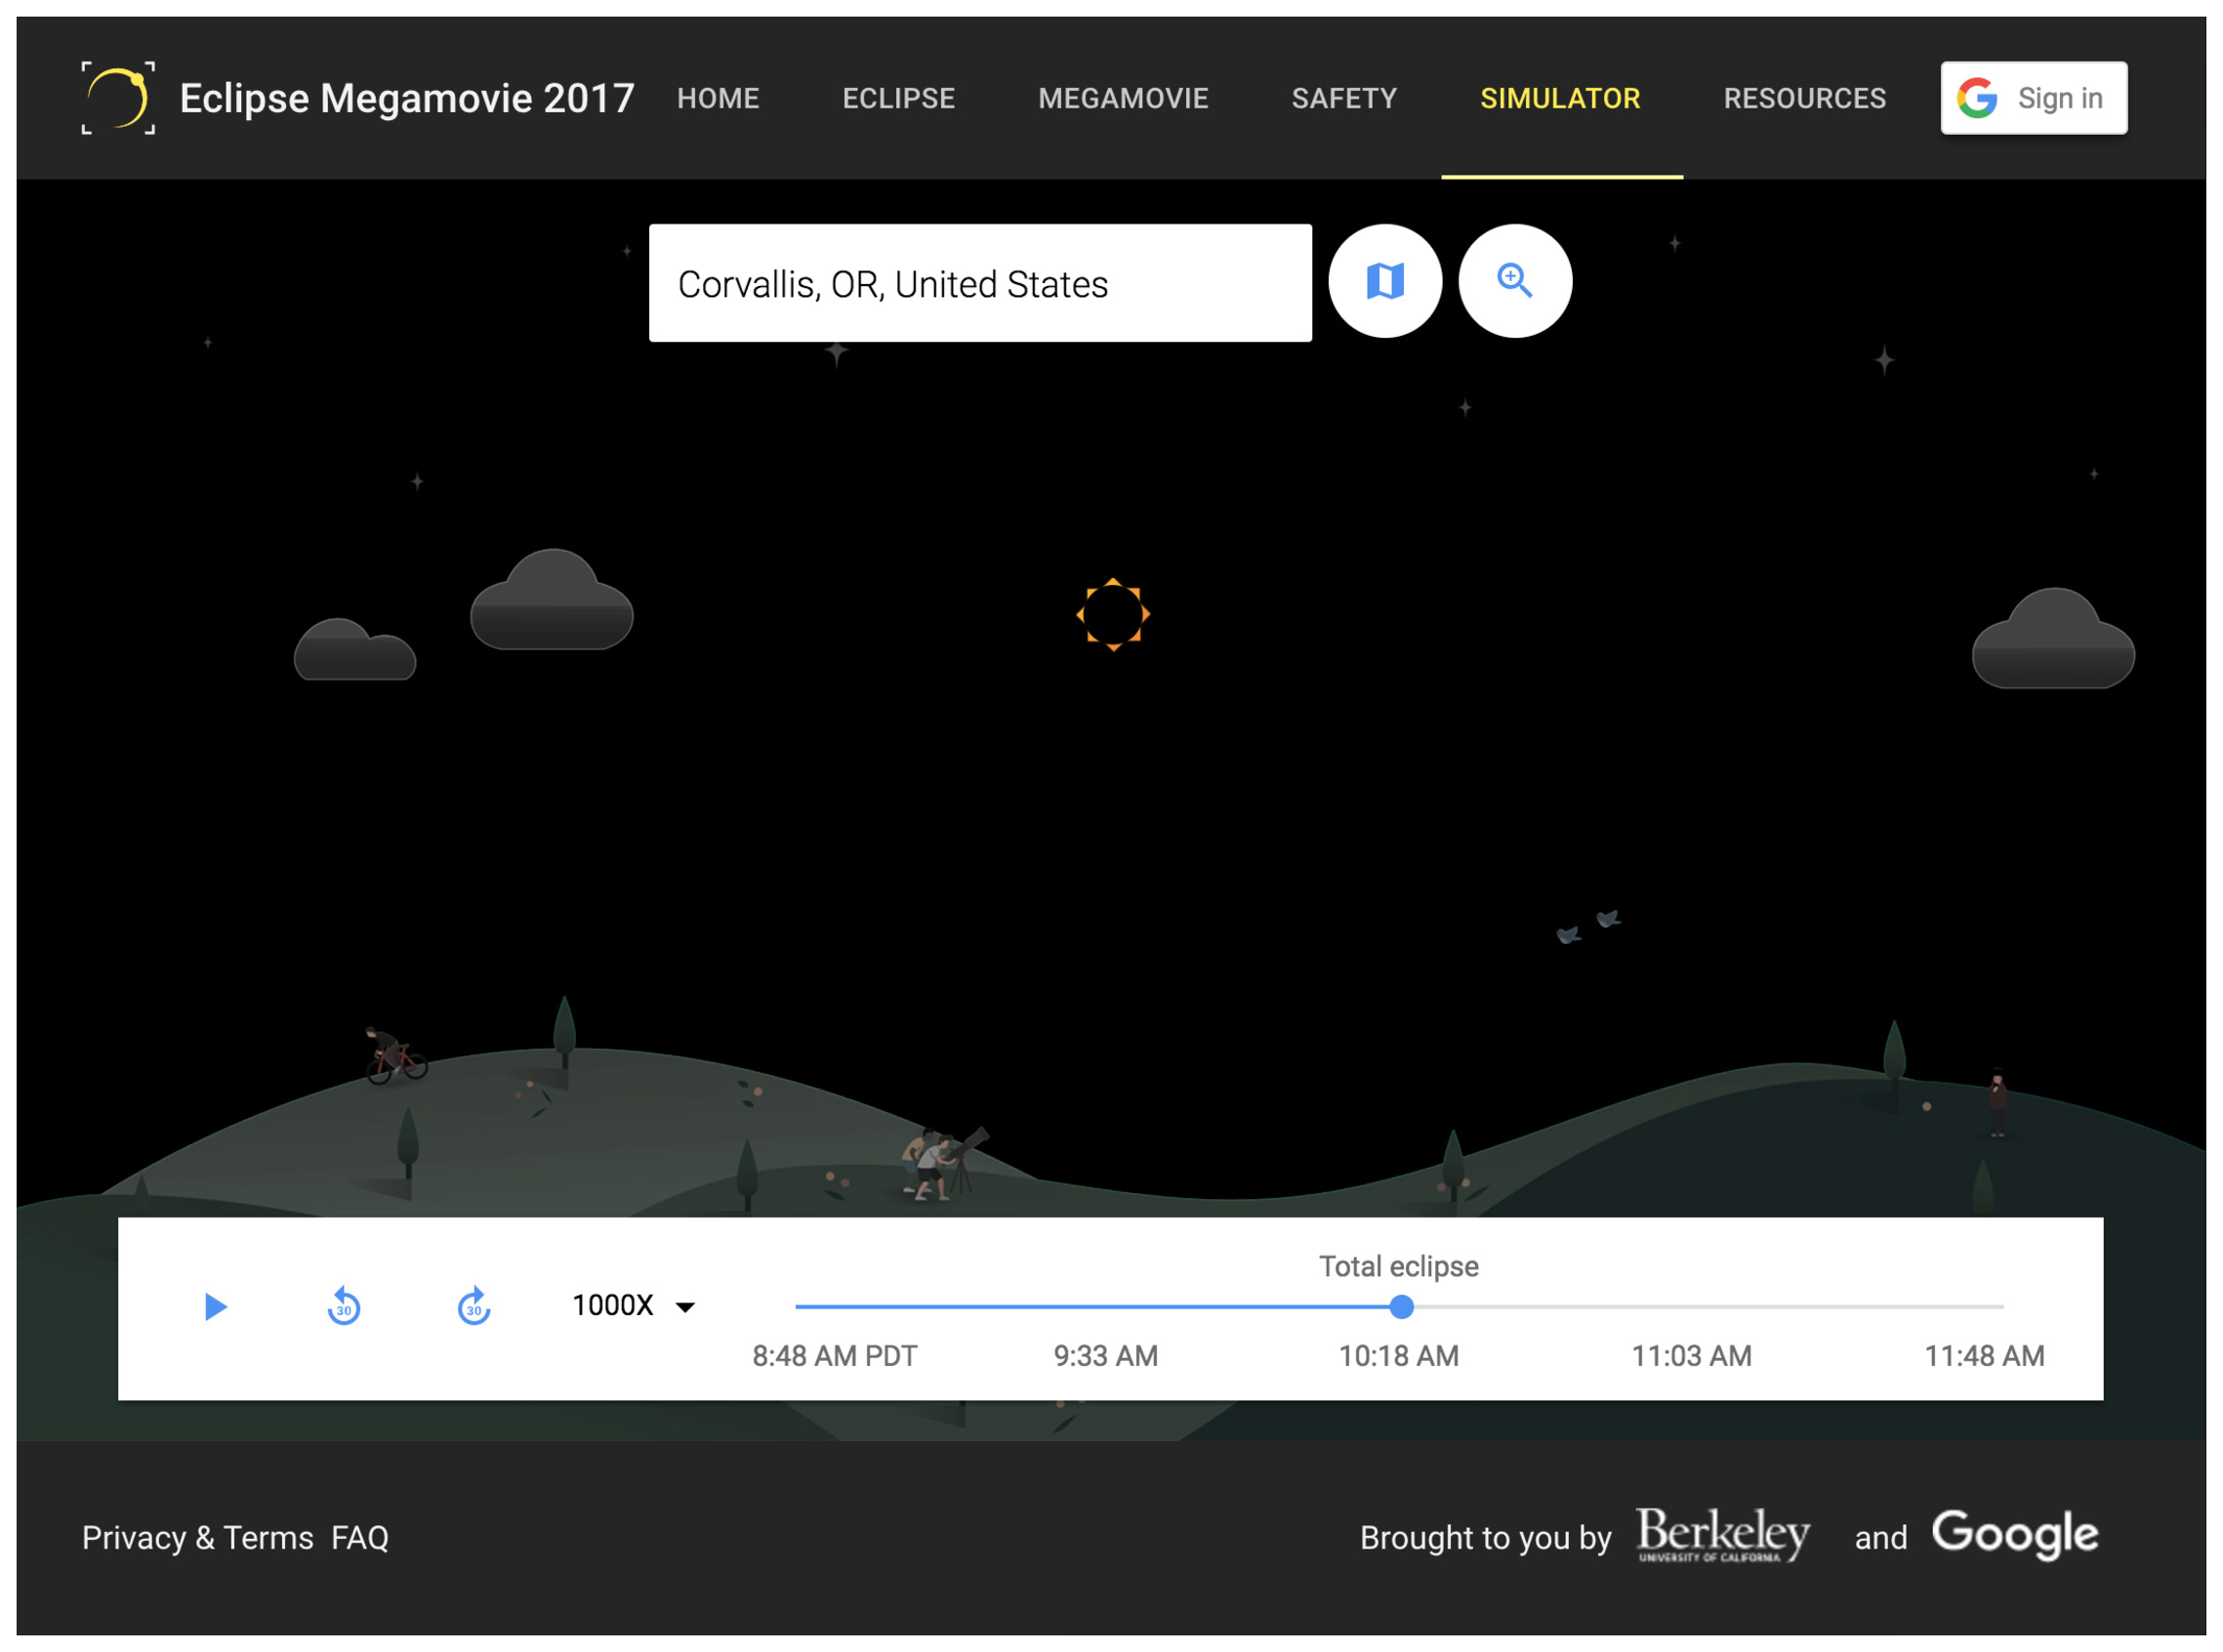
\includegraphics[width=\textwidth]{sim_total.eps}
		\caption{Simulator in wide mode showing a total solar eclipse}
	\end{center}
\end{figure}
\newpage

\begin{figure}[!h]
	\begin{center}
			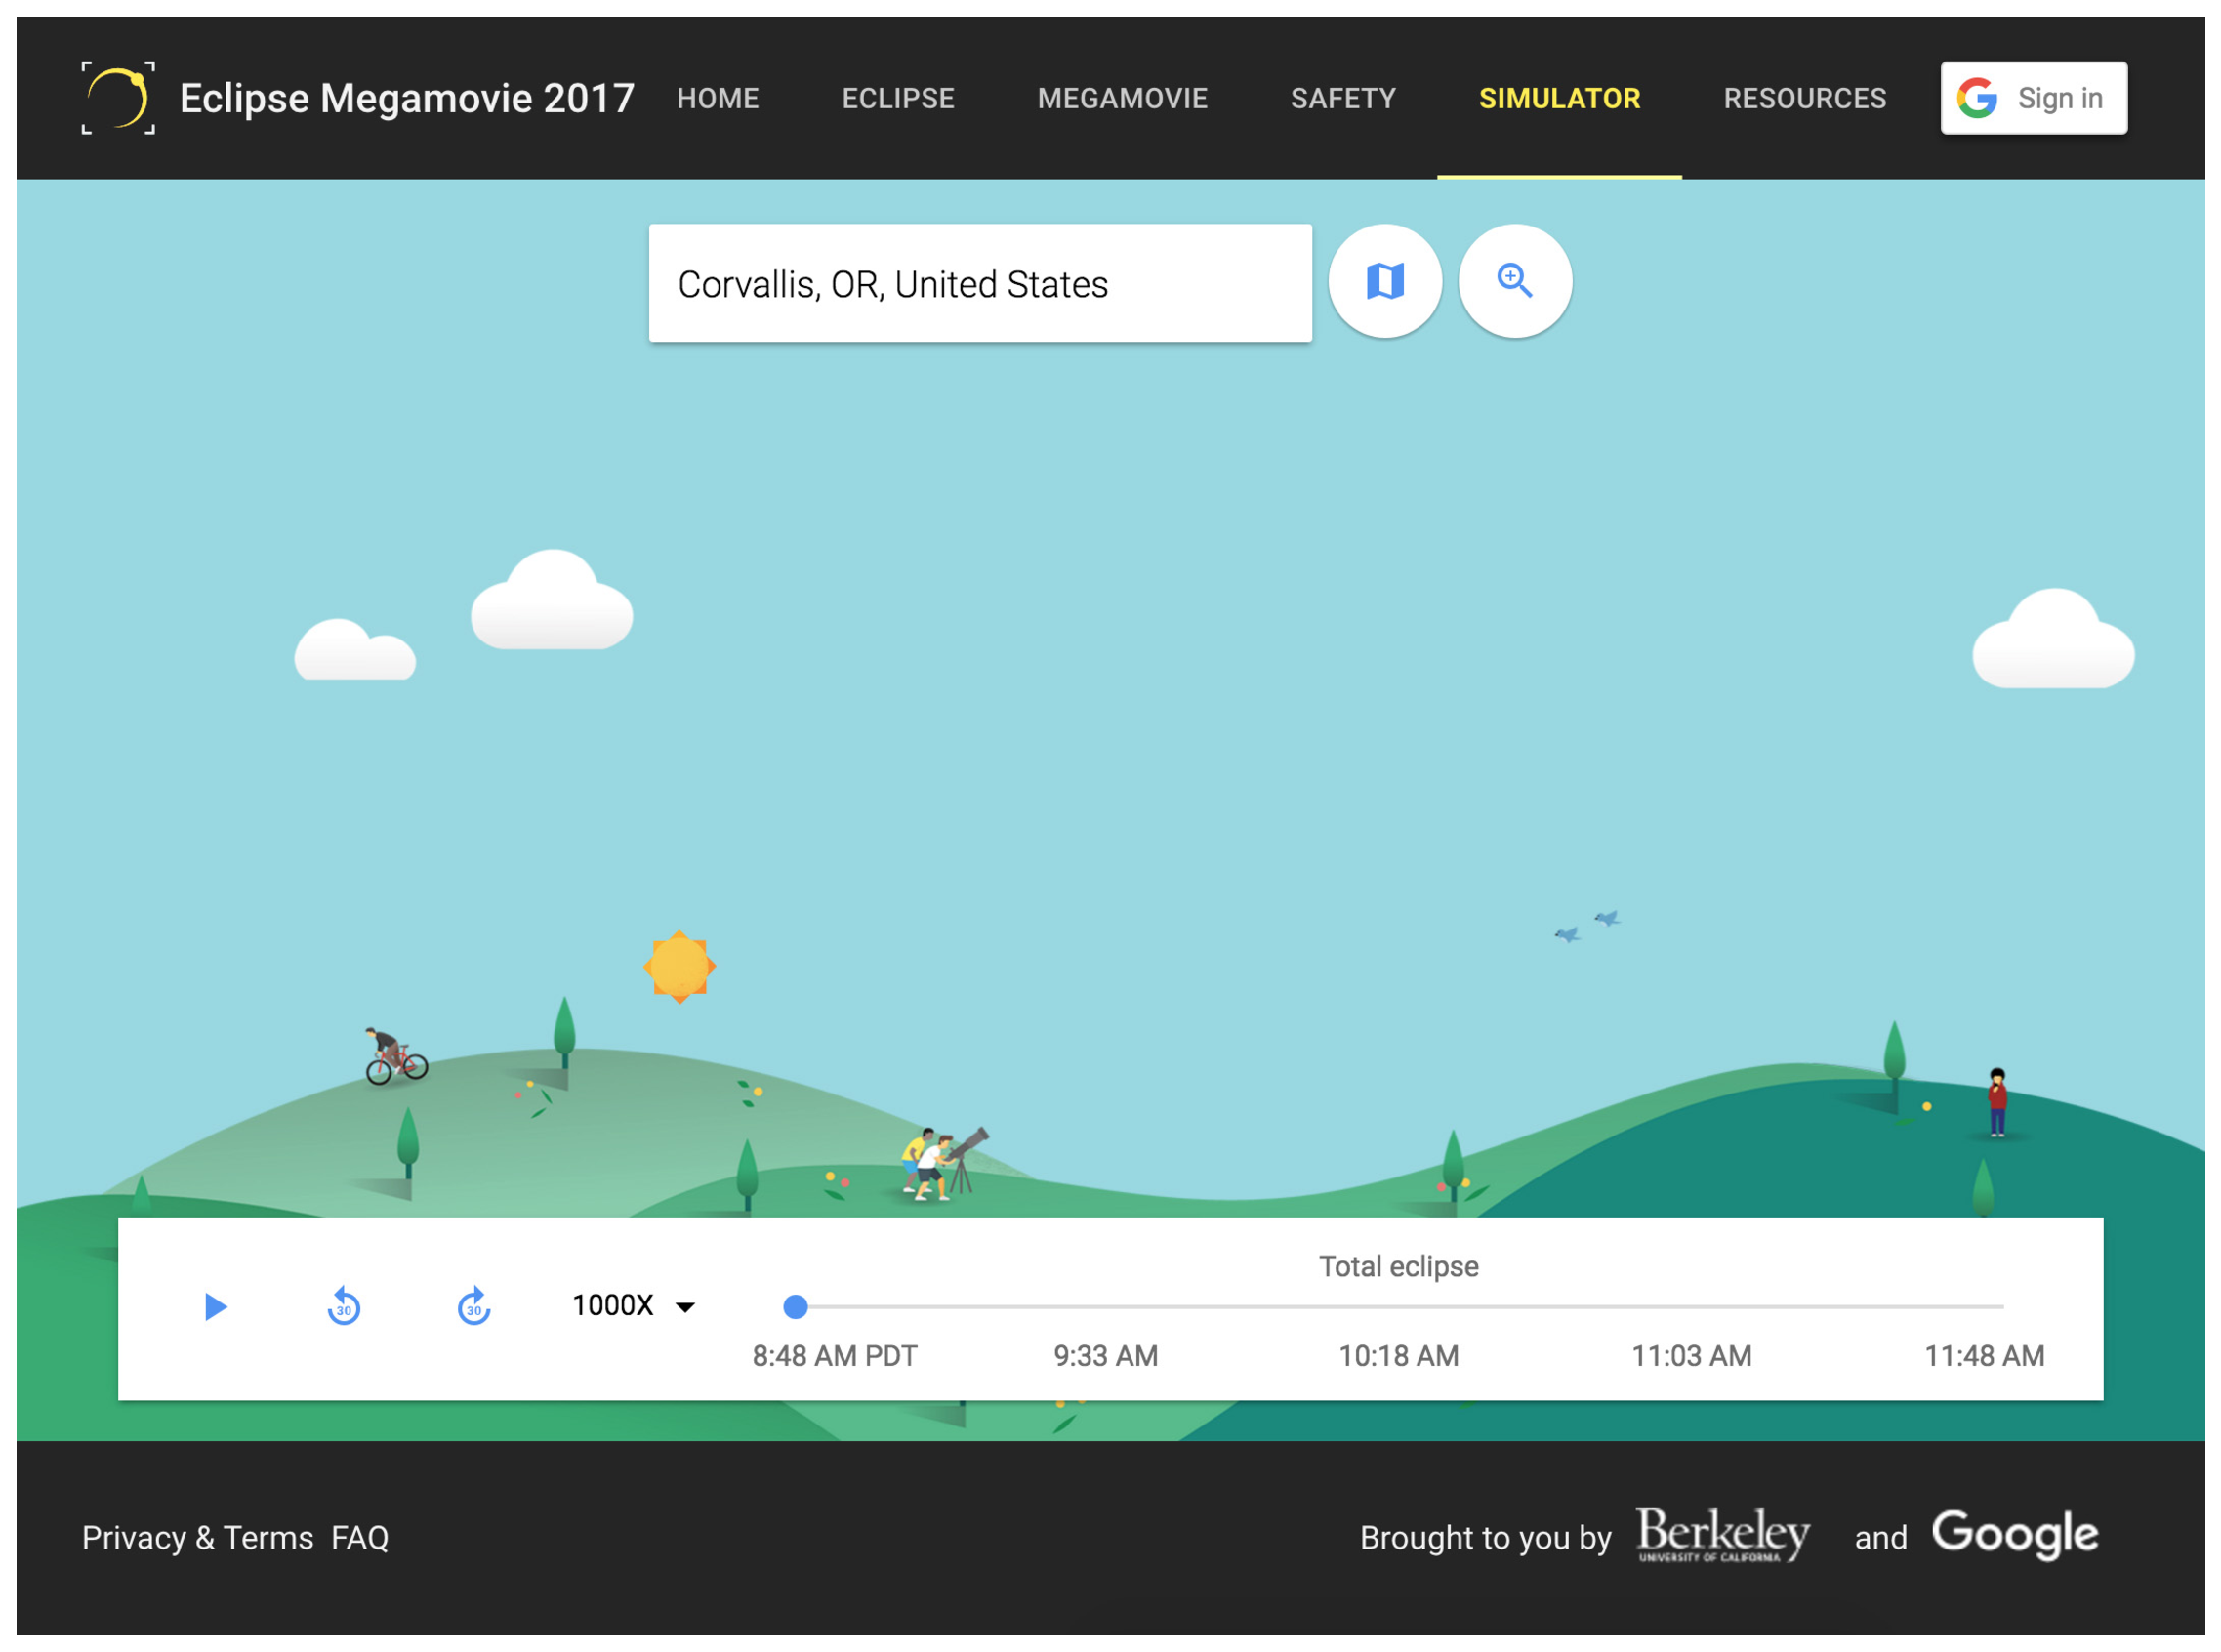
\includegraphics[width=\textwidth]{sim.eps}
		\caption{Simulator in wide mode showing no eclipse}
	\end{center}
\end{figure}
\newpage

\begin{figure}[!h]
	\begin{center}
			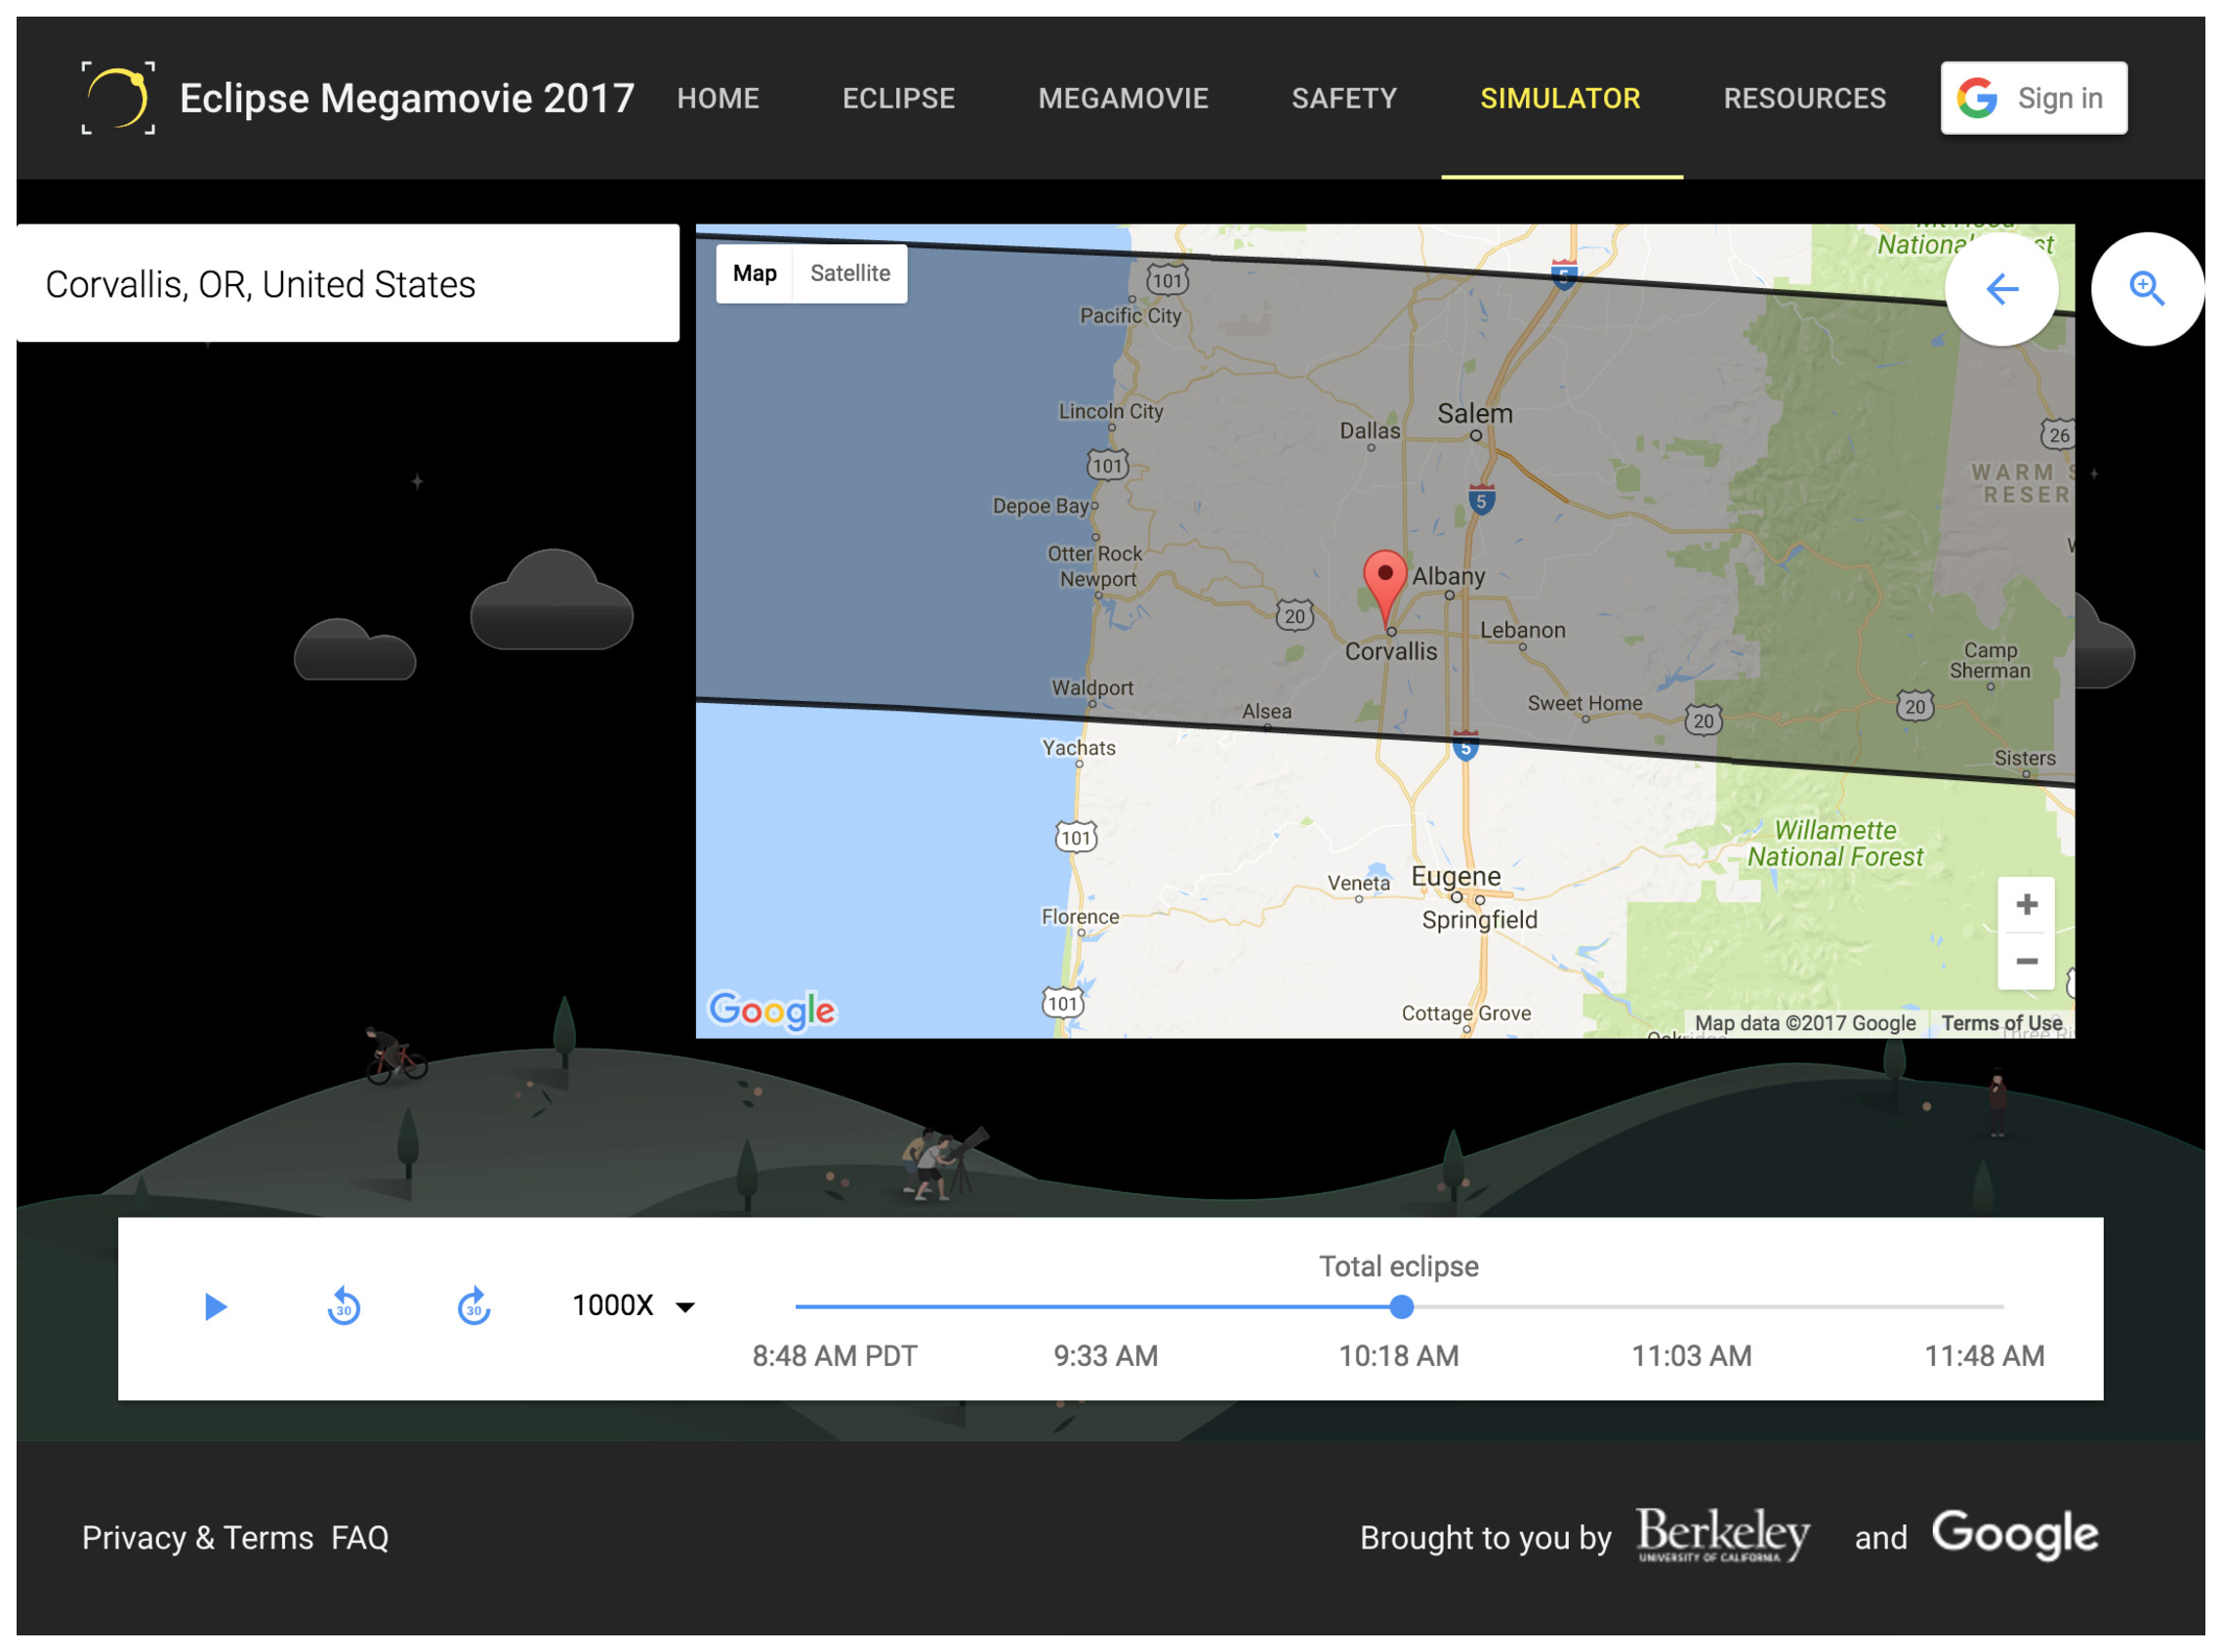
\includegraphics[width=\textwidth]{sim_map.eps}
		\caption{Simulator with map expanded}
	\end{center}
\end{figure}
\newpage

\begin{figure}[!h]
    \begin{center}
            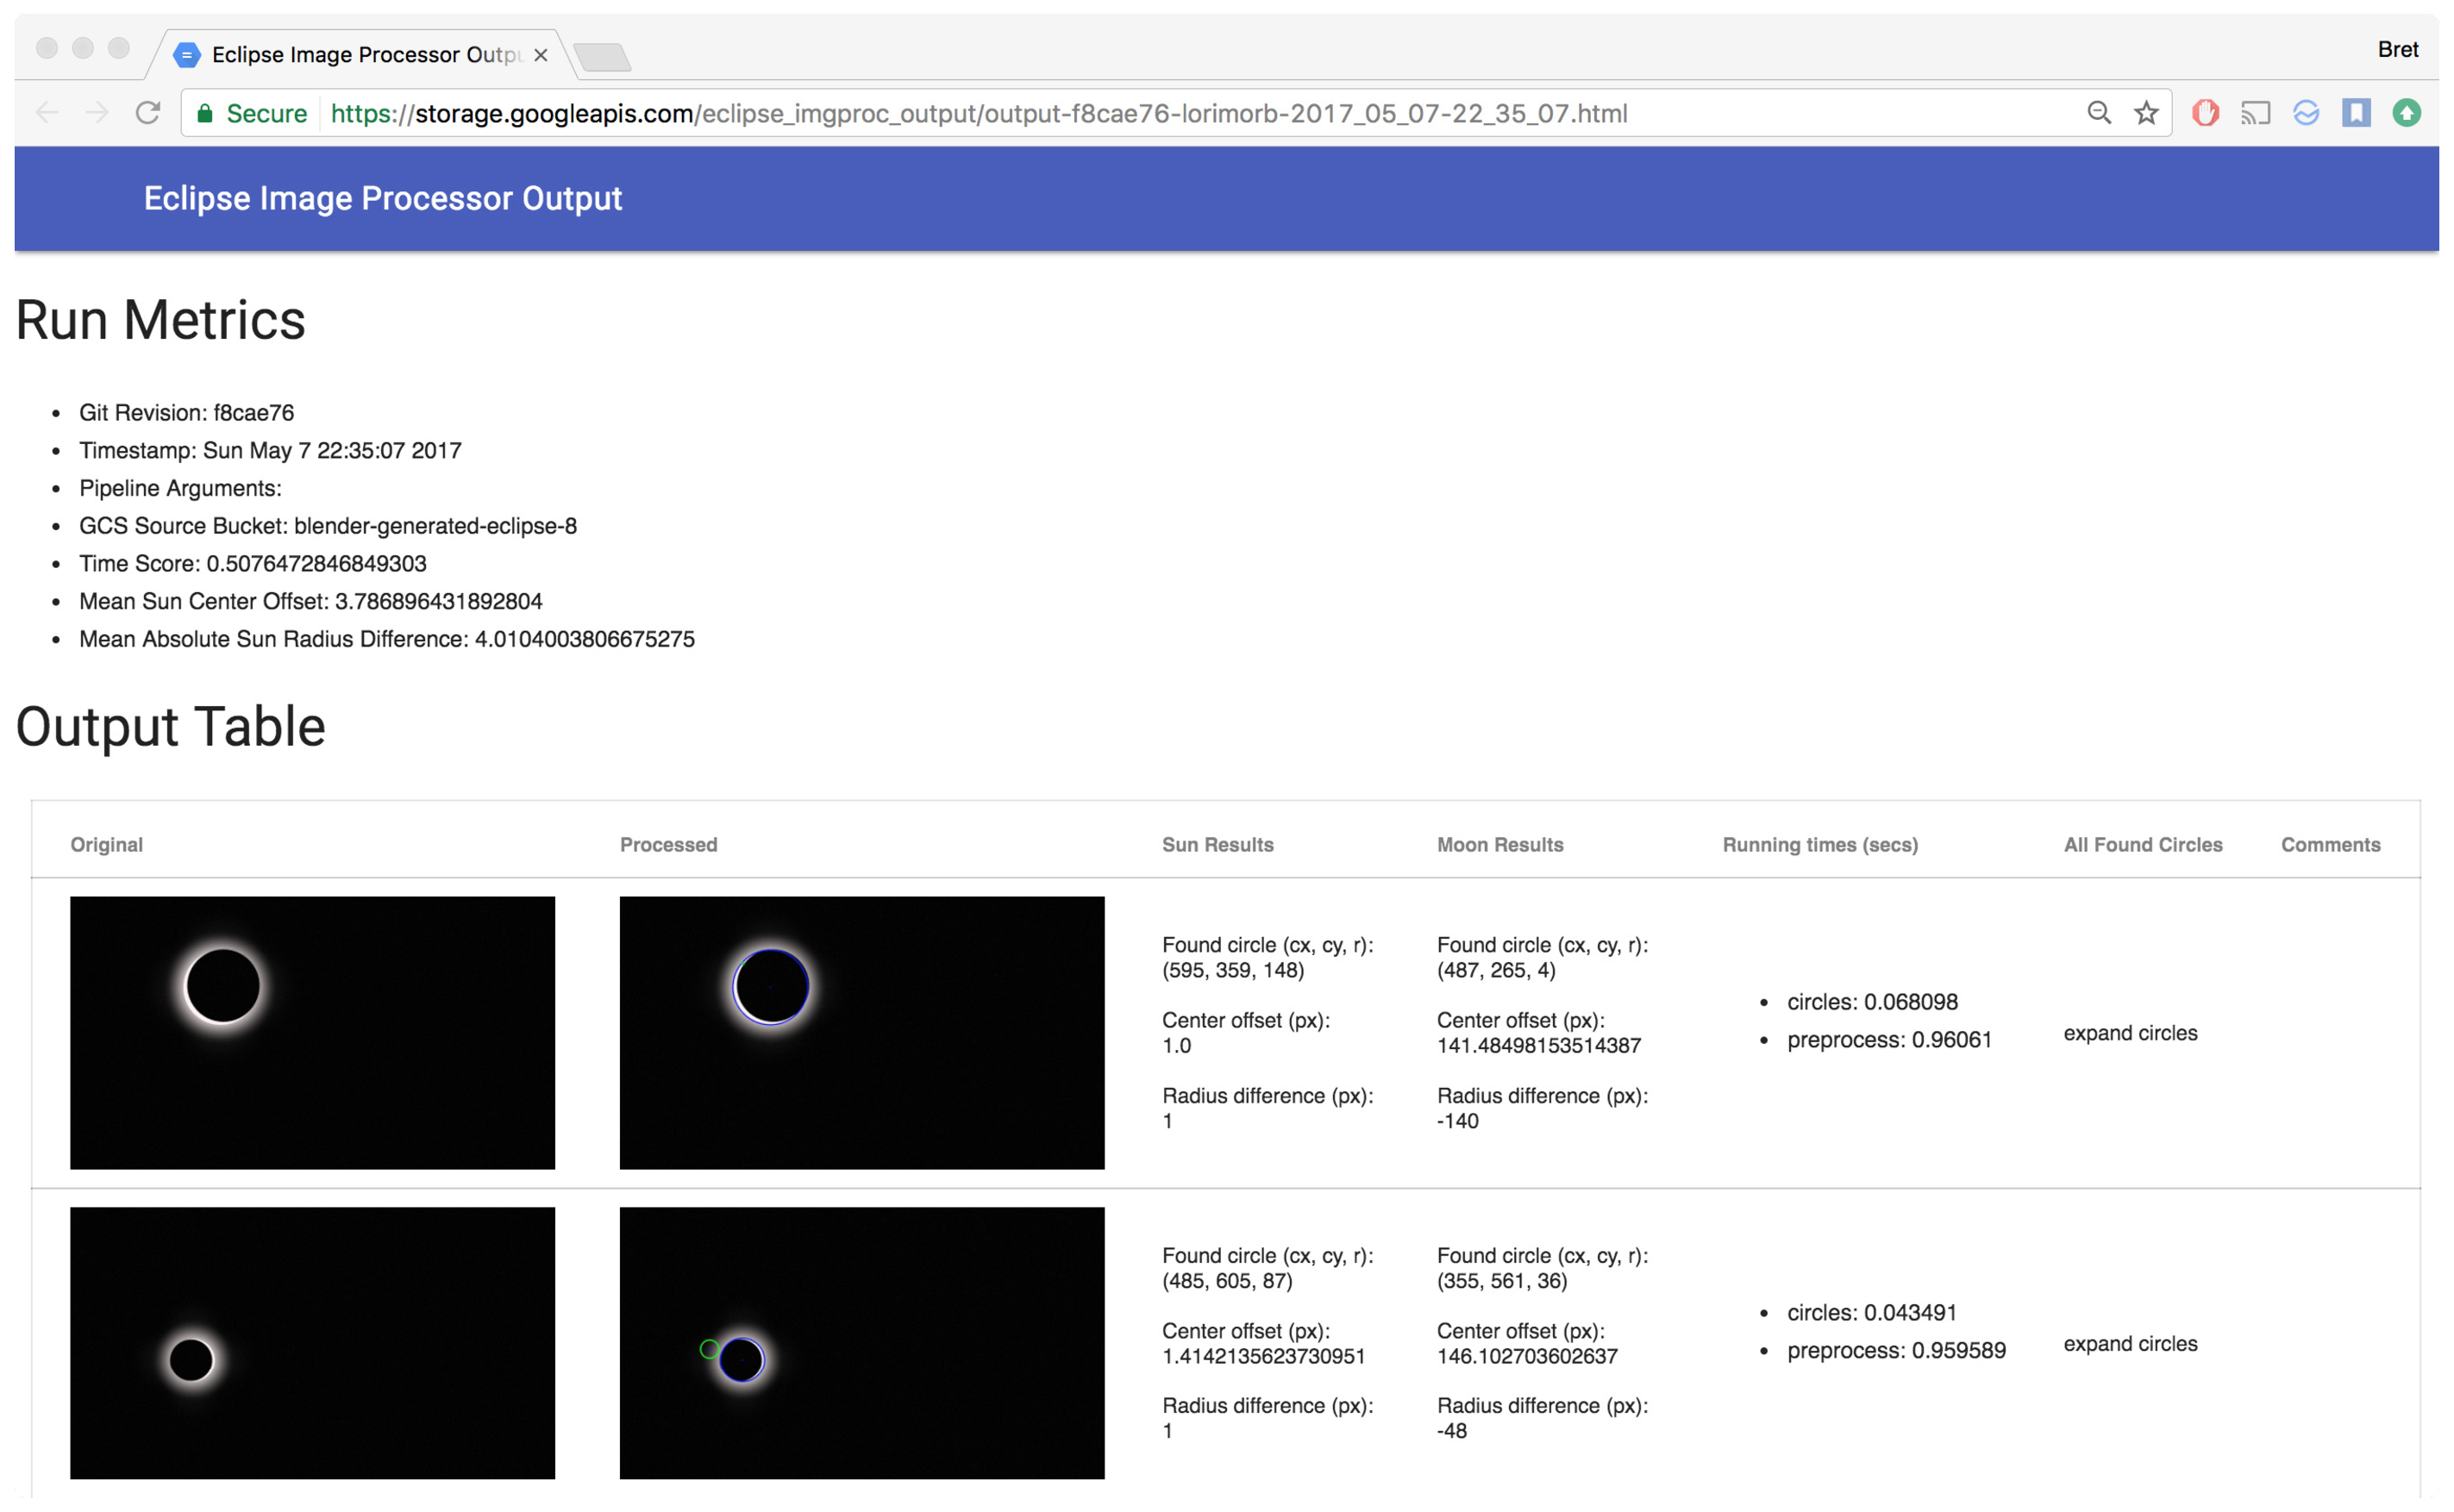
\includegraphics[width=\textwidth]{imgproc.eps}
        \caption{Image Processor Developer Pipeline Results File}
    \end{center}
\end{figure}
\newpage


%%%%%%%%%%%%%%%%%%%%%%%%
%   Weekly Summary     %
%%%%%%%%%%%%%%%%%%%%%%%%
\newpage
\section{Week by Week Summary of Group Activities}

\subsection{Week 1}

    \begin{itemize}

	\item Lorem

    \end{itemize}

\subsection{Week 2}

    \begin{itemize}

	\item Lorem

    \end{itemize}

\subsection{Week 3}

    \begin{itemize}

	\item Lorem

    \end{itemize}

\subsection{Week 4}

    \begin{itemize}

	\item Lorem

    \end{itemize}

\subsection{Week 5}

    \begin{itemize}

	\item Lorem

    \end{itemize}

\subsection{Week 6}

    \begin{itemize}

	\item Lorem

    \end{itemize}

\newpage
\section{Retrospectives}

\begin{table}[!h]
    \centering
    \begin{tabular}{|p{.3\linewidth}|p{.3\linewidth}|p{.3\linewidth}|}

    \cline{3-3}

    \hline \textbf{Positives} & \textbf{Deltas} & \textbf{Actions} \\ \hline

    Lorem & Lorem & Lorem \\ \hline

    \end{tabular}
\end{table}

\end{document}